% Created by tikzDevice version 0.7.0 on 2014-07-29 12:44:13
% !TEX encoding = UTF-8 Unicode
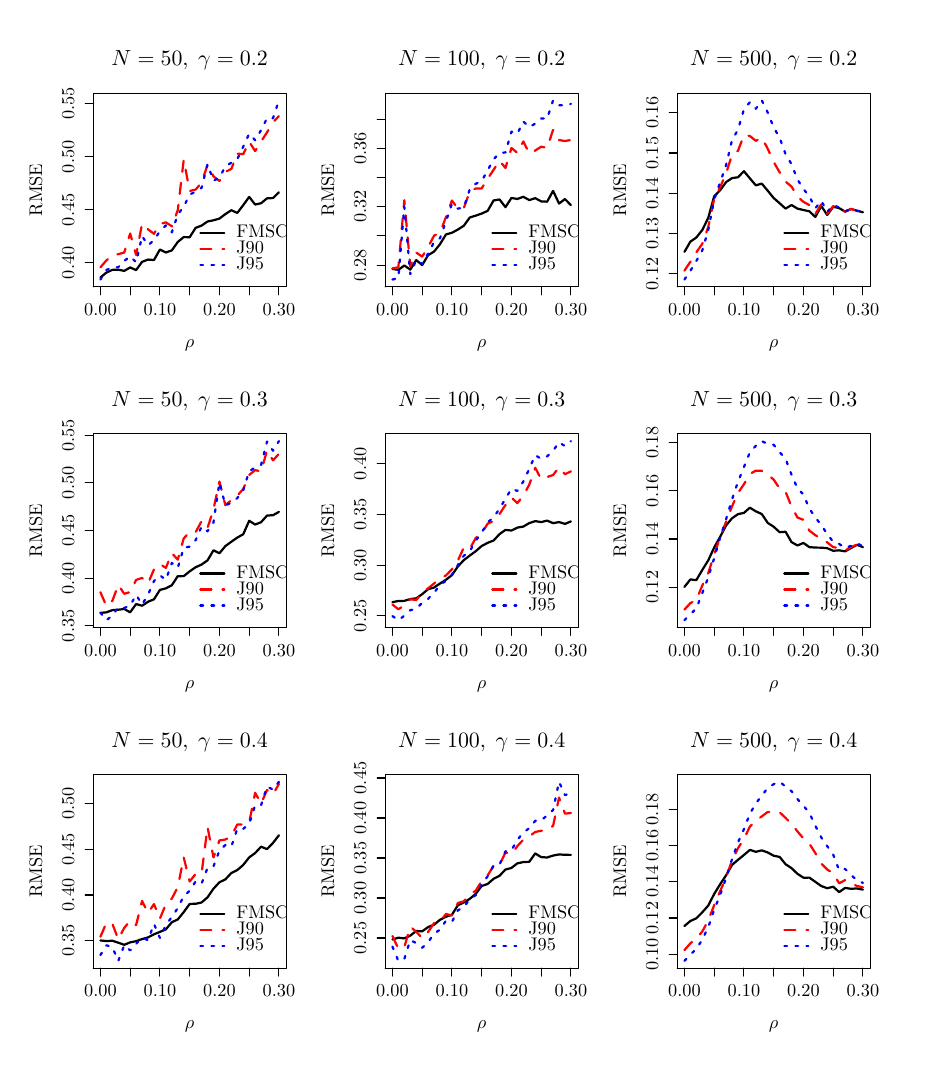
\begin{tikzpicture}[x=1pt,y=1pt,scale=0.73]
\definecolor[named]{fillColor}{rgb}{1.00,1.00,1.00}
\path[use as bounding box,fill=fillColor,fill opacity=0.00] (0,0) rectangle (433.62,505.89);
\begin{scope}
\path[clip] ( 32.47,377.65) rectangle (127.91,473.42);
\definecolor[named]{drawColor}{rgb}{0.00,0.00,0.00}

\path[draw=drawColor,line width= 0.8pt,line join=round,line cap=round] ( 36.01,382.24) --
	( 38.95,384.64) --
	( 41.90,386.00) --
	( 44.84,386.09) --
	( 47.79,385.49) --
	( 50.73,387.20) --
	( 53.68,385.90) --
	( 56.63,389.96) --
	( 59.57,391.10) --
	( 62.52,390.86) --
	( 65.46,396.08) --
	( 68.41,394.60) --
	( 71.35,395.63) --
	( 74.30,399.82) --
	( 77.24,402.22) --
	( 80.19,402.17) --
	( 83.14,406.79) --
	( 86.08,407.92) --
	( 89.03,409.94) --
	( 91.97,410.53) --
	( 94.92,411.38) --
	( 97.86,413.61) --
	(100.81,415.53) --
	(103.75,414.17) --
	(106.70,418.04) --
	(109.65,422.12) --
	(112.59,418.33) --
	(115.54,418.98) --
	(118.48,421.42) --
	(121.43,421.54) --
	(124.37,424.40);
\end{scope}
\begin{scope}
\path[clip] (  0.00,  0.00) rectangle (433.62,505.89);
\definecolor[named]{drawColor}{rgb}{0.00,0.00,0.00}

\path[draw=drawColor,line width= 0.4pt,line join=round,line cap=round] ( 36.01,377.65) -- (124.37,377.65);

\path[draw=drawColor,line width= 0.4pt,line join=round,line cap=round] ( 36.01,377.65) -- ( 36.01,373.69);

\path[draw=drawColor,line width= 0.4pt,line join=round,line cap=round] ( 50.73,377.65) -- ( 50.73,373.69);

\path[draw=drawColor,line width= 0.4pt,line join=round,line cap=round] ( 65.46,377.65) -- ( 65.46,373.69);

\path[draw=drawColor,line width= 0.4pt,line join=round,line cap=round] ( 80.19,377.65) -- ( 80.19,373.69);

\path[draw=drawColor,line width= 0.4pt,line join=round,line cap=round] ( 94.92,377.65) -- ( 94.92,373.69);

\path[draw=drawColor,line width= 0.4pt,line join=round,line cap=round] (109.65,377.65) -- (109.65,373.69);

\path[draw=drawColor,line width= 0.4pt,line join=round,line cap=round] (124.37,377.65) -- (124.37,373.69);

\node[text=drawColor,anchor=base,inner sep=0pt, outer sep=0pt, scale=  0.66] at ( 36.01,363.40) {0.00};

\node[text=drawColor,anchor=base,inner sep=0pt, outer sep=0pt, scale=  0.66] at ( 65.46,363.40) {0.10};

\node[text=drawColor,anchor=base,inner sep=0pt, outer sep=0pt, scale=  0.66] at ( 94.92,363.40) {0.20};

\node[text=drawColor,anchor=base,inner sep=0pt, outer sep=0pt, scale=  0.66] at (124.37,363.40) {0.30};

\path[draw=drawColor,line width= 0.4pt,line join=round,line cap=round] ( 32.47,389.48) -- ( 32.47,468.24);

\path[draw=drawColor,line width= 0.4pt,line join=round,line cap=round] ( 32.47,389.48) -- ( 28.51,389.48);

\path[draw=drawColor,line width= 0.4pt,line join=round,line cap=round] ( 32.47,415.73) -- ( 28.51,415.73);

\path[draw=drawColor,line width= 0.4pt,line join=round,line cap=round] ( 32.47,441.98) -- ( 28.51,441.98);

\path[draw=drawColor,line width= 0.4pt,line join=round,line cap=round] ( 32.47,468.24) -- ( 28.51,468.24);

\node[text=drawColor,rotate= 90.00,anchor=base,inner sep=0pt, outer sep=0pt, scale=  0.66] at ( 22.97,389.48) {0.40};

\node[text=drawColor,rotate= 90.00,anchor=base,inner sep=0pt, outer sep=0pt, scale=  0.66] at ( 22.97,415.73) {0.45};

\node[text=drawColor,rotate= 90.00,anchor=base,inner sep=0pt, outer sep=0pt, scale=  0.66] at ( 22.97,441.98) {0.50};

\node[text=drawColor,rotate= 90.00,anchor=base,inner sep=0pt, outer sep=0pt, scale=  0.66] at ( 22.97,468.24) {0.55};

\path[draw=drawColor,line width= 0.4pt,line join=round,line cap=round] ( 32.47,377.65) --
	(127.91,377.65) --
	(127.91,473.42) --
	( 32.47,473.42) --
	( 32.47,377.65);
\end{scope}
\begin{scope}
\path[clip] (  0.00,337.26) rectangle (144.54,505.89);
\definecolor[named]{drawColor}{rgb}{0.00,0.00,0.00}

\node[text=drawColor,anchor=base,inner sep=0pt, outer sep=0pt, scale=  0.79] at ( 80.19,486.92) {\bfseries $N=50, \;\gamma=0.2$};

\node[text=drawColor,anchor=base,inner sep=0pt, outer sep=0pt, scale=  0.66] at ( 80.19,347.56) {$\rho$};

\node[text=drawColor,rotate= 90.00,anchor=base,inner sep=0pt, outer sep=0pt, scale=  0.66] at (  7.13,425.53) {RMSE};
\end{scope}
\begin{scope}
\path[clip] ( 32.47,377.65) rectangle (127.91,473.42);
\definecolor[named]{drawColor}{rgb}{1.00,0.00,0.00}

\path[draw=drawColor,line width= 0.8pt,dash pattern=on 4pt off 4pt ,line join=round,line cap=round] ( 36.01,387.23) --
	( 38.95,390.68) --
	( 41.90,393.12) --
	( 44.84,393.77) --
	( 47.79,394.57) --
	( 50.73,404.00) --
	( 53.68,393.40) --
	( 56.63,408.86) --
	( 59.57,406.06) --
	( 62.52,403.85) --
	( 65.46,408.64) --
	( 68.41,409.52) --
	( 71.35,407.57) --
	( 74.30,415.54) --
	( 77.24,440.47) --
	( 80.19,425.03) --
	( 83.14,425.75) --
	( 86.08,429.15) --
	( 89.03,438.01) --
	( 91.97,432.29) --
	( 94.92,430.02) --
	( 97.86,434.47) --
	(100.81,435.96) --
	(103.75,443.54) --
	(106.70,443.27) --
	(109.65,449.48) --
	(112.59,444.80) --
	(115.54,449.55) --
	(118.48,454.07) --
	(121.43,459.03) --
	(124.37,462.12);
\definecolor[named]{drawColor}{rgb}{0.00,0.00,1.00}

\path[draw=drawColor,line width= 0.8pt,dash pattern=on 1pt off 3pt ,line join=round,line cap=round] ( 36.01,381.20) --
	( 38.95,385.95) --
	( 41.90,387.15) --
	( 44.84,387.33) --
	( 47.79,390.40) --
	( 50.73,392.73) --
	( 53.68,389.74) --
	( 56.63,402.74) --
	( 59.57,398.18) --
	( 62.52,400.61) --
	( 65.46,405.18) --
	( 68.41,407.99) --
	( 71.35,404.57) --
	( 74.30,413.44) --
	( 77.24,417.26) --
	( 80.19,423.33) --
	( 83.14,424.64) --
	( 86.08,426.61) --
	( 89.03,438.29) --
	( 91.97,430.09) --
	( 94.92,431.71) --
	( 97.86,437.18) --
	(100.81,439.06) --
	(103.75,440.82) --
	(106.70,446.96) --
	(109.65,453.42) --
	(112.59,450.18) --
	(115.54,455.21) --
	(118.48,461.08) --
	(121.43,461.04) --
	(124.37,469.87);
\definecolor[named]{drawColor}{rgb}{0.00,0.00,0.00}

\path[draw=drawColor,line width= 0.8pt,line join=round,line cap=round] ( 85.47,404.28) -- ( 97.35,404.28);
\definecolor[named]{drawColor}{rgb}{1.00,0.00,0.00}

\path[draw=drawColor,line width= 0.8pt,dash pattern=on 4pt off 4pt ,line join=round,line cap=round] ( 85.47,396.36) -- ( 97.35,396.36);
\definecolor[named]{drawColor}{rgb}{0.00,0.00,1.00}

\path[draw=drawColor,line width= 0.8pt,dash pattern=on 1pt off 3pt ,line join=round,line cap=round] ( 85.47,388.44) -- ( 97.35,388.44);
\definecolor[named]{drawColor}{rgb}{0.00,0.00,0.00}

\node[text=drawColor,anchor=base west,inner sep=0pt, outer sep=0pt, scale=  0.66] at (103.29,402.01) {FMSC};

\node[text=drawColor,anchor=base west,inner sep=0pt, outer sep=0pt, scale=  0.66] at (103.29,394.09) {J90};

\node[text=drawColor,anchor=base west,inner sep=0pt, outer sep=0pt, scale=  0.66] at (103.29,386.17) {J95};
\end{scope}
\begin{scope}
\path[clip] (177.01,377.65) rectangle (272.45,473.42);
\definecolor[named]{drawColor}{rgb}{0.00,0.00,0.00}

\path[draw=drawColor,line width= 0.8pt,line join=round,line cap=round] (180.55,386.45) --
	(183.49,386.00) --
	(186.44,388.16) --
	(189.38,386.12) --
	(192.33,390.86) --
	(195.27,388.37) --
	(198.22,393.26) --
	(201.17,395.07) --
	(204.11,398.73) --
	(207.06,403.54) --
	(210.00,404.35) --
	(212.95,405.96) --
	(215.89,407.84) --
	(218.84,411.92) --
	(221.78,412.85) --
	(224.73,413.86) --
	(227.68,415.20) --
	(230.62,420.35) --
	(233.57,420.84) --
	(236.51,417.04) --
	(239.46,421.60) --
	(242.40,421.09) --
	(245.35,422.19) --
	(248.29,420.54) --
	(251.24,421.48) --
	(254.19,419.89) --
	(257.13,419.75) --
	(260.08,425.10) --
	(263.02,418.83) --
	(265.97,421.05) --
	(268.91,418.00);
\end{scope}
\begin{scope}
\path[clip] (  0.00,  0.00) rectangle (433.62,505.89);
\definecolor[named]{drawColor}{rgb}{0.00,0.00,0.00}

\path[draw=drawColor,line width= 0.4pt,line join=round,line cap=round] (180.55,377.65) -- (268.91,377.65);

\path[draw=drawColor,line width= 0.4pt,line join=round,line cap=round] (180.55,377.65) -- (180.55,373.69);

\path[draw=drawColor,line width= 0.4pt,line join=round,line cap=round] (195.27,377.65) -- (195.27,373.69);

\path[draw=drawColor,line width= 0.4pt,line join=round,line cap=round] (210.00,377.65) -- (210.00,373.69);

\path[draw=drawColor,line width= 0.4pt,line join=round,line cap=round] (224.73,377.65) -- (224.73,373.69);

\path[draw=drawColor,line width= 0.4pt,line join=round,line cap=round] (239.46,377.65) -- (239.46,373.69);

\path[draw=drawColor,line width= 0.4pt,line join=round,line cap=round] (254.19,377.65) -- (254.19,373.69);

\path[draw=drawColor,line width= 0.4pt,line join=round,line cap=round] (268.91,377.65) -- (268.91,373.69);

\node[text=drawColor,anchor=base,inner sep=0pt, outer sep=0pt, scale=  0.66] at (180.55,363.40) {0.00};

\node[text=drawColor,anchor=base,inner sep=0pt, outer sep=0pt, scale=  0.66] at (210.00,363.40) {0.10};

\node[text=drawColor,anchor=base,inner sep=0pt, outer sep=0pt, scale=  0.66] at (239.46,363.40) {0.20};

\node[text=drawColor,anchor=base,inner sep=0pt, outer sep=0pt, scale=  0.66] at (268.91,363.40) {0.30};

\path[draw=drawColor,line width= 0.4pt,line join=round,line cap=round] (177.01,388.33) -- (177.01,460.64);

\path[draw=drawColor,line width= 0.4pt,line join=round,line cap=round] (177.01,388.33) -- (173.05,388.33);

\path[draw=drawColor,line width= 0.4pt,line join=round,line cap=round] (177.01,402.79) -- (173.05,402.79);

\path[draw=drawColor,line width= 0.4pt,line join=round,line cap=round] (177.01,417.26) -- (173.05,417.26);

\path[draw=drawColor,line width= 0.4pt,line join=round,line cap=round] (177.01,431.72) -- (173.05,431.72);

\path[draw=drawColor,line width= 0.4pt,line join=round,line cap=round] (177.01,446.18) -- (173.05,446.18);

\path[draw=drawColor,line width= 0.4pt,line join=round,line cap=round] (177.01,460.64) -- (173.05,460.64);

\node[text=drawColor,rotate= 90.00,anchor=base,inner sep=0pt, outer sep=0pt, scale=  0.66] at (167.51,388.33) {0.28};

\node[text=drawColor,rotate= 90.00,anchor=base,inner sep=0pt, outer sep=0pt, scale=  0.66] at (167.51,417.26) {0.32};

\node[text=drawColor,rotate= 90.00,anchor=base,inner sep=0pt, outer sep=0pt, scale=  0.66] at (167.51,446.18) {0.36};

\path[draw=drawColor,line width= 0.4pt,line join=round,line cap=round] (177.01,377.65) --
	(272.45,377.65) --
	(272.45,473.42) --
	(177.01,473.42) --
	(177.01,377.65);
\end{scope}
\begin{scope}
\path[clip] (144.54,337.26) rectangle (289.08,505.89);
\definecolor[named]{drawColor}{rgb}{0.00,0.00,0.00}

\node[text=drawColor,anchor=base,inner sep=0pt, outer sep=0pt, scale=  0.79] at (224.73,486.92) {\bfseries $N=100, \;\gamma=0.2$};

\node[text=drawColor,anchor=base,inner sep=0pt, outer sep=0pt, scale=  0.66] at (224.73,347.56) {$\rho$};

\node[text=drawColor,rotate= 90.00,anchor=base,inner sep=0pt, outer sep=0pt, scale=  0.66] at (151.67,425.53) {RMSE};
\end{scope}
\begin{scope}
\path[clip] (177.01,377.65) rectangle (272.45,473.42);
\definecolor[named]{drawColor}{rgb}{1.00,0.00,0.00}

\path[draw=drawColor,line width= 0.8pt,dash pattern=on 4pt off 4pt ,line join=round,line cap=round] (180.55,386.74) --
	(183.49,387.28) --
	(186.44,420.48) --
	(189.38,387.75) --
	(192.33,394.57) --
	(195.27,392.54) --
	(198.22,397.31) --
	(201.17,402.93) --
	(204.11,404.50) --
	(207.06,412.13) --
	(210.00,420.30) --
	(212.95,416.32) --
	(215.89,416.63) --
	(218.84,424.83) --
	(221.78,426.26) --
	(224.73,426.33) --
	(227.68,431.11) --
	(230.62,435.52) --
	(233.57,440.06) --
	(236.51,436.42) --
	(239.46,446.35) --
	(242.40,443.91) --
	(245.35,449.58) --
	(248.29,443.66) --
	(251.24,445.06) --
	(254.19,446.98) --
	(257.13,446.39) --
	(260.08,455.25) --
	(263.02,450.26) --
	(265.97,449.79) --
	(268.91,450.29);
\definecolor[named]{drawColor}{rgb}{0.00,0.00,1.00}

\path[draw=drawColor,line width= 0.8pt,dash pattern=on 1pt off 3pt ,line join=round,line cap=round] (180.55,381.20) --
	(183.49,381.89) --
	(186.44,417.28) --
	(189.38,383.89) --
	(192.33,390.89) --
	(195.27,388.96) --
	(198.22,394.14) --
	(201.17,399.75) --
	(204.11,401.69) --
	(207.06,410.07) --
	(210.00,418.71) --
	(212.95,416.30) --
	(215.89,416.85) --
	(218.84,425.88) --
	(221.78,428.61) --
	(224.73,429.98) --
	(227.68,435.26) --
	(230.62,440.72) --
	(233.57,443.85) --
	(236.51,444.11) --
	(239.46,454.43) --
	(242.40,453.45) --
	(245.35,459.42) --
	(248.29,456.70) --
	(251.24,458.38) --
	(254.19,460.96) --
	(257.13,460.87) --
	(260.08,469.87) --
	(263.02,467.44) --
	(265.97,467.60) --
	(268.91,468.18);
\definecolor[named]{drawColor}{rgb}{0.00,0.00,0.00}

\path[draw=drawColor,line width= 0.8pt,line join=round,line cap=round] (230.01,404.28) -- (241.89,404.28);
\definecolor[named]{drawColor}{rgb}{1.00,0.00,0.00}

\path[draw=drawColor,line width= 0.8pt,dash pattern=on 4pt off 4pt ,line join=round,line cap=round] (230.01,396.36) -- (241.89,396.36);
\definecolor[named]{drawColor}{rgb}{0.00,0.00,1.00}

\path[draw=drawColor,line width= 0.8pt,dash pattern=on 1pt off 3pt ,line join=round,line cap=round] (230.01,388.44) -- (241.89,388.44);
\definecolor[named]{drawColor}{rgb}{0.00,0.00,0.00}

\node[text=drawColor,anchor=base west,inner sep=0pt, outer sep=0pt, scale=  0.66] at (247.83,402.01) {FMSC};

\node[text=drawColor,anchor=base west,inner sep=0pt, outer sep=0pt, scale=  0.66] at (247.83,394.09) {J90};

\node[text=drawColor,anchor=base west,inner sep=0pt, outer sep=0pt, scale=  0.66] at (247.83,386.17) {J95};
\end{scope}
\begin{scope}
\path[clip] (321.55,377.65) rectangle (416.99,473.42);
\definecolor[named]{drawColor}{rgb}{0.00,0.00,0.00}

\path[draw=drawColor,line width= 0.8pt,line join=round,line cap=round] (325.09,394.90) --
	(328.03,399.96) --
	(330.98,402.01) --
	(333.92,405.72) --
	(336.87,411.69) --
	(339.81,422.39) --
	(342.76,425.41) --
	(345.71,429.44) --
	(348.65,431.43) --
	(351.60,431.83) --
	(354.54,434.85) --
	(357.49,431.30) --
	(360.43,427.84) --
	(363.38,428.70) --
	(366.32,425.19) --
	(369.27,421.56) --
	(372.22,418.97) --
	(375.16,416.32) --
	(378.11,418.09) --
	(381.05,416.31) --
	(384.00,415.63) --
	(386.94,414.99) --
	(389.89,412.17) --
	(392.83,417.62) --
	(395.78,413.15) --
	(398.73,417.23) --
	(401.67,416.58) --
	(404.62,414.83) --
	(407.56,416.13) --
	(410.51,415.27) --
	(413.45,414.53);
\end{scope}
\begin{scope}
\path[clip] (  0.00,  0.00) rectangle (433.62,505.89);
\definecolor[named]{drawColor}{rgb}{0.00,0.00,0.00}

\path[draw=drawColor,line width= 0.4pt,line join=round,line cap=round] (325.09,377.65) -- (413.45,377.65);

\path[draw=drawColor,line width= 0.4pt,line join=round,line cap=round] (325.09,377.65) -- (325.09,373.69);

\path[draw=drawColor,line width= 0.4pt,line join=round,line cap=round] (339.81,377.65) -- (339.81,373.69);

\path[draw=drawColor,line width= 0.4pt,line join=round,line cap=round] (354.54,377.65) -- (354.54,373.69);

\path[draw=drawColor,line width= 0.4pt,line join=round,line cap=round] (369.27,377.65) -- (369.27,373.69);

\path[draw=drawColor,line width= 0.4pt,line join=round,line cap=round] (384.00,377.65) -- (384.00,373.69);

\path[draw=drawColor,line width= 0.4pt,line join=round,line cap=round] (398.73,377.65) -- (398.73,373.69);

\path[draw=drawColor,line width= 0.4pt,line join=round,line cap=round] (413.45,377.65) -- (413.45,373.69);

\node[text=drawColor,anchor=base,inner sep=0pt, outer sep=0pt, scale=  0.66] at (325.09,363.40) {0.00};

\node[text=drawColor,anchor=base,inner sep=0pt, outer sep=0pt, scale=  0.66] at (354.54,363.40) {0.10};

\node[text=drawColor,anchor=base,inner sep=0pt, outer sep=0pt, scale=  0.66] at (384.00,363.40) {0.20};

\node[text=drawColor,anchor=base,inner sep=0pt, outer sep=0pt, scale=  0.66] at (413.45,363.40) {0.30};

\path[draw=drawColor,line width= 0.4pt,line join=round,line cap=round] (321.55,383.98) -- (321.55,463.82);

\path[draw=drawColor,line width= 0.4pt,line join=round,line cap=round] (321.55,383.98) -- (317.59,383.98);

\path[draw=drawColor,line width= 0.4pt,line join=round,line cap=round] (321.55,403.94) -- (317.59,403.94);

\path[draw=drawColor,line width= 0.4pt,line join=round,line cap=round] (321.55,423.90) -- (317.59,423.90);

\path[draw=drawColor,line width= 0.4pt,line join=round,line cap=round] (321.55,443.86) -- (317.59,443.86);

\path[draw=drawColor,line width= 0.4pt,line join=round,line cap=round] (321.55,463.82) -- (317.59,463.82);

\node[text=drawColor,rotate= 90.00,anchor=base,inner sep=0pt, outer sep=0pt, scale=  0.66] at (312.05,383.98) {0.12};

\node[text=drawColor,rotate= 90.00,anchor=base,inner sep=0pt, outer sep=0pt, scale=  0.66] at (312.05,403.94) {0.13};

\node[text=drawColor,rotate= 90.00,anchor=base,inner sep=0pt, outer sep=0pt, scale=  0.66] at (312.05,423.90) {0.14};

\node[text=drawColor,rotate= 90.00,anchor=base,inner sep=0pt, outer sep=0pt, scale=  0.66] at (312.05,443.86) {0.15};

\node[text=drawColor,rotate= 90.00,anchor=base,inner sep=0pt, outer sep=0pt, scale=  0.66] at (312.05,463.82) {0.16};

\path[draw=drawColor,line width= 0.4pt,line join=round,line cap=round] (321.55,377.65) --
	(416.99,377.65) --
	(416.99,473.42) --
	(321.55,473.42) --
	(321.55,377.65);
\end{scope}
\begin{scope}
\path[clip] (289.08,337.26) rectangle (433.62,505.89);
\definecolor[named]{drawColor}{rgb}{0.00,0.00,0.00}

\node[text=drawColor,anchor=base,inner sep=0pt, outer sep=0pt, scale=  0.79] at (369.27,486.92) {\bfseries $N=500, \;\gamma=0.2$};

\node[text=drawColor,anchor=base,inner sep=0pt, outer sep=0pt, scale=  0.66] at (369.27,347.56) {$\rho$};

\node[text=drawColor,rotate= 90.00,anchor=base,inner sep=0pt, outer sep=0pt, scale=  0.66] at (296.21,425.53) {RMSE};
\end{scope}
\begin{scope}
\path[clip] (321.55,377.65) rectangle (416.99,473.42);
\definecolor[named]{drawColor}{rgb}{1.00,0.00,0.00}

\path[draw=drawColor,line width= 0.8pt,dash pattern=on 4pt off 4pt ,line join=round,line cap=round] (325.09,385.60) --
	(328.03,389.98) --
	(330.98,394.70) --
	(333.92,398.87) --
	(336.87,407.17) --
	(339.81,421.11) --
	(342.76,426.90) --
	(345.71,433.79) --
	(348.65,442.99) --
	(351.60,444.95) --
	(354.54,452.63) --
	(357.49,452.27) --
	(360.43,449.86) --
	(363.38,451.38) --
	(366.32,445.99) --
	(369.27,439.37) --
	(372.22,434.30) --
	(375.16,429.68) --
	(378.11,427.23) --
	(381.05,422.28) --
	(384.00,419.67) --
	(386.94,418.04) --
	(389.89,413.68) --
	(392.83,418.49) --
	(395.78,413.75) --
	(398.73,417.57) --
	(401.67,416.67) --
	(404.62,414.86) --
	(407.56,416.13) --
	(410.51,415.27) --
	(413.45,414.53);
\definecolor[named]{drawColor}{rgb}{0.00,0.00,1.00}

\path[draw=drawColor,line width= 0.8pt,dash pattern=on 1pt off 3pt ,line join=round,line cap=round] (325.09,381.20) --
	(328.03,385.55) --
	(330.98,390.38) --
	(333.92,395.58) --
	(336.87,405.70) --
	(339.81,420.78) --
	(342.76,429.27) --
	(345.71,437.84) --
	(348.65,450.21) --
	(351.60,455.37) --
	(354.54,465.45) --
	(357.49,468.98) --
	(360.43,465.77) --
	(363.38,469.87) --
	(366.32,463.87) --
	(369.27,456.55) --
	(372.22,451.38) --
	(375.16,443.29) --
	(378.11,438.31) --
	(381.05,430.75) --
	(384.00,425.99) --
	(386.94,422.43) --
	(389.89,416.49) --
	(392.83,420.21) --
	(395.78,414.69) --
	(398.73,418.05) --
	(401.67,416.89) --
	(404.62,414.93) --
	(407.56,416.14) --
	(410.51,415.27) --
	(413.45,414.53);
\definecolor[named]{drawColor}{rgb}{0.00,0.00,0.00}

\path[draw=drawColor,line width= 0.8pt,line join=round,line cap=round] (374.55,404.28) -- (386.43,404.28);
\definecolor[named]{drawColor}{rgb}{1.00,0.00,0.00}

\path[draw=drawColor,line width= 0.8pt,dash pattern=on 4pt off 4pt ,line join=round,line cap=round] (374.55,396.36) -- (386.43,396.36);
\definecolor[named]{drawColor}{rgb}{0.00,0.00,1.00}

\path[draw=drawColor,line width= 0.8pt,dash pattern=on 1pt off 3pt ,line join=round,line cap=round] (374.55,388.44) -- (386.43,388.44);
\definecolor[named]{drawColor}{rgb}{0.00,0.00,0.00}

\node[text=drawColor,anchor=base west,inner sep=0pt, outer sep=0pt, scale=  0.66] at (392.37,402.01) {FMSC};

\node[text=drawColor,anchor=base west,inner sep=0pt, outer sep=0pt, scale=  0.66] at (392.37,394.09) {J90};

\node[text=drawColor,anchor=base west,inner sep=0pt, outer sep=0pt, scale=  0.66] at (392.37,386.17) {J95};
\end{scope}
\begin{scope}
\path[clip] ( 32.47,209.02) rectangle (127.91,304.79);
\definecolor[named]{drawColor}{rgb}{0.00,0.00,0.00}

\path[draw=drawColor,line width= 0.8pt,line join=round,line cap=round] ( 36.01,216.20) --
	( 38.95,216.48) --
	( 41.90,217.56) --
	( 44.84,217.77) --
	( 47.79,218.15) --
	( 50.73,216.49) --
	( 53.68,220.58) --
	( 56.63,219.75) --
	( 59.57,221.72) --
	( 62.52,222.93) --
	( 65.46,227.58) --
	( 68.41,228.35) --
	( 71.35,229.90) --
	( 74.30,234.38) --
	( 77.24,234.40) --
	( 80.19,236.77) --
	( 83.14,238.80) --
	( 86.08,240.12) --
	( 89.03,242.21) --
	( 91.97,247.17) --
	( 94.92,245.73) --
	( 97.86,249.25) --
	(100.81,251.43) --
	(103.75,253.47) --
	(106.70,255.13) --
	(109.65,261.81) --
	(112.59,259.93) --
	(115.54,261.10) --
	(118.48,264.38) --
	(121.43,264.56) --
	(124.37,266.20);
\end{scope}
\begin{scope}
\path[clip] (  0.00,  0.00) rectangle (433.62,505.89);
\definecolor[named]{drawColor}{rgb}{0.00,0.00,0.00}

\path[draw=drawColor,line width= 0.4pt,line join=round,line cap=round] ( 36.01,209.02) -- (124.37,209.02);

\path[draw=drawColor,line width= 0.4pt,line join=round,line cap=round] ( 36.01,209.02) -- ( 36.01,205.06);

\path[draw=drawColor,line width= 0.4pt,line join=round,line cap=round] ( 50.73,209.02) -- ( 50.73,205.06);

\path[draw=drawColor,line width= 0.4pt,line join=round,line cap=round] ( 65.46,209.02) -- ( 65.46,205.06);

\path[draw=drawColor,line width= 0.4pt,line join=round,line cap=round] ( 80.19,209.02) -- ( 80.19,205.06);

\path[draw=drawColor,line width= 0.4pt,line join=round,line cap=round] ( 94.92,209.02) -- ( 94.92,205.06);

\path[draw=drawColor,line width= 0.4pt,line join=round,line cap=round] (109.65,209.02) -- (109.65,205.06);

\path[draw=drawColor,line width= 0.4pt,line join=round,line cap=round] (124.37,209.02) -- (124.37,205.06);

\node[text=drawColor,anchor=base,inner sep=0pt, outer sep=0pt, scale=  0.66] at ( 36.01,194.77) {0.00};

\node[text=drawColor,anchor=base,inner sep=0pt, outer sep=0pt, scale=  0.66] at ( 65.46,194.77) {0.10};

\node[text=drawColor,anchor=base,inner sep=0pt, outer sep=0pt, scale=  0.66] at ( 94.92,194.77) {0.20};

\node[text=drawColor,anchor=base,inner sep=0pt, outer sep=0pt, scale=  0.66] at (124.37,194.77) {0.30};

\path[draw=drawColor,line width= 0.4pt,line join=round,line cap=round] ( 32.47,209.80) -- ( 32.47,304.16);

\path[draw=drawColor,line width= 0.4pt,line join=round,line cap=round] ( 32.47,209.80) -- ( 28.51,209.80);

\path[draw=drawColor,line width= 0.4pt,line join=round,line cap=round] ( 32.47,233.39) -- ( 28.51,233.39);

\path[draw=drawColor,line width= 0.4pt,line join=round,line cap=round] ( 32.47,256.98) -- ( 28.51,256.98);

\path[draw=drawColor,line width= 0.4pt,line join=round,line cap=round] ( 32.47,280.57) -- ( 28.51,280.57);

\path[draw=drawColor,line width= 0.4pt,line join=round,line cap=round] ( 32.47,304.16) -- ( 28.51,304.16);

\node[text=drawColor,rotate= 90.00,anchor=base,inner sep=0pt, outer sep=0pt, scale=  0.66] at ( 22.97,209.80) {0.35};

\node[text=drawColor,rotate= 90.00,anchor=base,inner sep=0pt, outer sep=0pt, scale=  0.66] at ( 22.97,233.39) {0.40};

\node[text=drawColor,rotate= 90.00,anchor=base,inner sep=0pt, outer sep=0pt, scale=  0.66] at ( 22.97,256.98) {0.45};

\node[text=drawColor,rotate= 90.00,anchor=base,inner sep=0pt, outer sep=0pt, scale=  0.66] at ( 22.97,280.57) {0.50};

\node[text=drawColor,rotate= 90.00,anchor=base,inner sep=0pt, outer sep=0pt, scale=  0.66] at ( 22.97,304.16) {0.55};

\path[draw=drawColor,line width= 0.4pt,line join=round,line cap=round] ( 32.47,209.02) --
	(127.91,209.02) --
	(127.91,304.79) --
	( 32.47,304.79) --
	( 32.47,209.02);
\end{scope}
\begin{scope}
\path[clip] (  0.00,168.63) rectangle (144.54,337.26);
\definecolor[named]{drawColor}{rgb}{0.00,0.00,0.00}

\node[text=drawColor,anchor=base,inner sep=0pt, outer sep=0pt, scale=  0.79] at ( 80.19,318.29) {\bfseries $N=50, \;\gamma=0.3$};

\node[text=drawColor,anchor=base,inner sep=0pt, outer sep=0pt, scale=  0.66] at ( 80.19,178.93) {$\rho$};

\node[text=drawColor,rotate= 90.00,anchor=base,inner sep=0pt, outer sep=0pt, scale=  0.66] at (  7.13,256.90) {RMSE};
\end{scope}
\begin{scope}
\path[clip] ( 32.47,209.02) rectangle (127.91,304.79);
\definecolor[named]{drawColor}{rgb}{1.00,0.00,0.00}

\path[draw=drawColor,line width= 0.8pt,dash pattern=on 4pt off 4pt ,line join=round,line cap=round] ( 36.01,226.42) --
	( 38.95,219.64) --
	( 41.90,222.11) --
	( 44.84,230.05) --
	( 47.79,225.66) --
	( 50.73,226.52) --
	( 53.68,232.51) --
	( 56.63,233.49) --
	( 59.57,230.78) --
	( 62.52,237.74) --
	( 65.46,240.39) --
	( 68.41,238.47) --
	( 71.35,245.79) --
	( 74.30,242.55) --
	( 77.24,253.03) --
	( 80.19,256.32) --
	( 83.14,256.16) --
	( 86.08,261.59) --
	( 89.03,258.23) --
	( 91.97,267.50) --
	( 94.92,281.22) --
	( 97.86,269.51) --
	(100.81,272.04) --
	(103.75,274.21) --
	(106.70,277.54) --
	(109.65,284.47) --
	(112.59,286.88) --
	(115.54,286.18) --
	(118.48,296.62) --
	(121.43,291.70) --
	(124.37,294.94);
\definecolor[named]{drawColor}{rgb}{0.00,0.00,1.00}

\path[draw=drawColor,line width= 0.8pt,dash pattern=on 1pt off 3pt ,line join=round,line cap=round] ( 36.01,216.34) --
	( 38.95,212.57) --
	( 41.90,214.80) --
	( 44.84,219.00) --
	( 47.79,218.67) --
	( 50.73,219.74) --
	( 53.68,225.14) --
	( 56.63,220.36) --
	( 59.57,225.18) --
	( 62.52,231.98) --
	( 65.46,234.77) --
	( 68.41,232.62) --
	( 71.35,240.92) --
	( 74.30,238.50) --
	( 77.24,248.39) --
	( 80.19,249.02) --
	( 83.14,252.21) --
	( 86.08,258.95) --
	( 89.03,256.60) --
	( 91.97,260.97) --
	( 94.92,280.76) --
	( 97.86,269.46) --
	(100.81,270.71) --
	(103.75,273.02) --
	(106.70,276.96) --
	(109.65,286.32) --
	(112.59,288.21) --
	(115.54,289.46) --
	(118.48,301.02) --
	(121.43,296.47) --
	(124.37,301.24);
\definecolor[named]{drawColor}{rgb}{0.00,0.00,0.00}

\path[draw=drawColor,line width= 0.8pt,line join=round,line cap=round] ( 85.47,235.65) -- ( 97.35,235.65);
\definecolor[named]{drawColor}{rgb}{1.00,0.00,0.00}

\path[draw=drawColor,line width= 0.8pt,dash pattern=on 4pt off 4pt ,line join=round,line cap=round] ( 85.47,227.73) -- ( 97.35,227.73);
\definecolor[named]{drawColor}{rgb}{0.00,0.00,1.00}

\path[draw=drawColor,line width= 0.8pt,dash pattern=on 1pt off 3pt ,line join=round,line cap=round] ( 85.47,219.81) -- ( 97.35,219.81);
\definecolor[named]{drawColor}{rgb}{0.00,0.00,0.00}

\node[text=drawColor,anchor=base west,inner sep=0pt, outer sep=0pt, scale=  0.66] at (103.29,233.38) {FMSC};

\node[text=drawColor,anchor=base west,inner sep=0pt, outer sep=0pt, scale=  0.66] at (103.29,225.46) {J90};

\node[text=drawColor,anchor=base west,inner sep=0pt, outer sep=0pt, scale=  0.66] at (103.29,217.54) {J95};
\end{scope}
\begin{scope}
\path[clip] (177.01,209.02) rectangle (272.45,304.79);
\definecolor[named]{drawColor}{rgb}{0.00,0.00,0.00}

\path[draw=drawColor,line width= 0.8pt,line join=round,line cap=round] (180.55,221.52) --
	(183.49,222.09) --
	(186.44,222.15) --
	(189.38,223.05) --
	(192.33,223.40) --
	(195.27,225.45) --
	(198.22,227.97) --
	(201.17,228.75) --
	(204.11,230.75) --
	(207.06,232.62) --
	(210.00,234.89) --
	(212.95,239.20) --
	(215.89,242.32) --
	(218.84,244.57) --
	(221.78,246.73) --
	(224.73,249.30) --
	(227.68,250.88) --
	(230.62,252.02) --
	(233.57,255.20) --
	(236.51,257.28) --
	(239.46,256.97) --
	(242.40,258.42) --
	(245.35,258.93) --
	(248.29,260.65) --
	(251.24,261.64) --
	(254.19,261.14) --
	(257.13,261.89) --
	(260.08,260.61) --
	(263.02,261.16) --
	(265.97,260.27) --
	(268.91,261.48);
\end{scope}
\begin{scope}
\path[clip] (  0.00,  0.00) rectangle (433.62,505.89);
\definecolor[named]{drawColor}{rgb}{0.00,0.00,0.00}

\path[draw=drawColor,line width= 0.4pt,line join=round,line cap=round] (180.55,209.02) -- (268.91,209.02);

\path[draw=drawColor,line width= 0.4pt,line join=round,line cap=round] (180.55,209.02) -- (180.55,205.06);

\path[draw=drawColor,line width= 0.4pt,line join=round,line cap=round] (195.27,209.02) -- (195.27,205.06);

\path[draw=drawColor,line width= 0.4pt,line join=round,line cap=round] (210.00,209.02) -- (210.00,205.06);

\path[draw=drawColor,line width= 0.4pt,line join=round,line cap=round] (224.73,209.02) -- (224.73,205.06);

\path[draw=drawColor,line width= 0.4pt,line join=round,line cap=round] (239.46,209.02) -- (239.46,205.06);

\path[draw=drawColor,line width= 0.4pt,line join=round,line cap=round] (254.19,209.02) -- (254.19,205.06);

\path[draw=drawColor,line width= 0.4pt,line join=round,line cap=round] (268.91,209.02) -- (268.91,205.06);

\node[text=drawColor,anchor=base,inner sep=0pt, outer sep=0pt, scale=  0.66] at (180.55,194.77) {0.00};

\node[text=drawColor,anchor=base,inner sep=0pt, outer sep=0pt, scale=  0.66] at (210.00,194.77) {0.10};

\node[text=drawColor,anchor=base,inner sep=0pt, outer sep=0pt, scale=  0.66] at (239.46,194.77) {0.20};

\node[text=drawColor,anchor=base,inner sep=0pt, outer sep=0pt, scale=  0.66] at (268.91,194.77) {0.30};

\path[draw=drawColor,line width= 0.4pt,line join=round,line cap=round] (177.01,214.77) -- (177.01,290.02);

\path[draw=drawColor,line width= 0.4pt,line join=round,line cap=round] (177.01,214.77) -- (173.05,214.77);

\path[draw=drawColor,line width= 0.4pt,line join=round,line cap=round] (177.01,239.85) -- (173.05,239.85);

\path[draw=drawColor,line width= 0.4pt,line join=round,line cap=round] (177.01,264.93) -- (173.05,264.93);

\path[draw=drawColor,line width= 0.4pt,line join=round,line cap=round] (177.01,290.02) -- (173.05,290.02);

\node[text=drawColor,rotate= 90.00,anchor=base,inner sep=0pt, outer sep=0pt, scale=  0.66] at (167.51,214.77) {0.25};

\node[text=drawColor,rotate= 90.00,anchor=base,inner sep=0pt, outer sep=0pt, scale=  0.66] at (167.51,239.85) {0.30};

\node[text=drawColor,rotate= 90.00,anchor=base,inner sep=0pt, outer sep=0pt, scale=  0.66] at (167.51,264.93) {0.35};

\node[text=drawColor,rotate= 90.00,anchor=base,inner sep=0pt, outer sep=0pt, scale=  0.66] at (167.51,290.02) {0.40};

\path[draw=drawColor,line width= 0.4pt,line join=round,line cap=round] (177.01,209.02) --
	(272.45,209.02) --
	(272.45,304.79) --
	(177.01,304.79) --
	(177.01,209.02);
\end{scope}
\begin{scope}
\path[clip] (144.54,168.63) rectangle (289.08,337.26);
\definecolor[named]{drawColor}{rgb}{0.00,0.00,0.00}

\node[text=drawColor,anchor=base,inner sep=0pt, outer sep=0pt, scale=  0.79] at (224.73,318.29) {\bfseries $N=100, \;\gamma=0.3$};

\node[text=drawColor,anchor=base,inner sep=0pt, outer sep=0pt, scale=  0.66] at (224.73,178.93) {$\rho$};

\node[text=drawColor,rotate= 90.00,anchor=base,inner sep=0pt, outer sep=0pt, scale=  0.66] at (151.67,256.90) {RMSE};
\end{scope}
\begin{scope}
\path[clip] (177.01,209.02) rectangle (272.45,304.79);
\definecolor[named]{drawColor}{rgb}{1.00,0.00,0.00}

\path[draw=drawColor,line width= 0.8pt,dash pattern=on 4pt off 4pt ,line join=round,line cap=round] (180.55,220.36) --
	(183.49,217.98) --
	(186.44,219.99) --
	(189.38,222.93) --
	(192.33,222.59) --
	(195.27,226.03) --
	(198.22,228.35) --
	(201.17,230.79) --
	(204.11,233.18) --
	(207.06,234.74) --
	(210.00,237.79) --
	(212.95,242.10) --
	(215.89,248.58) --
	(218.84,247.85) --
	(221.78,253.28) --
	(224.73,255.43) --
	(227.68,260.38) --
	(230.62,261.62) --
	(233.57,265.17) --
	(236.51,269.60) --
	(239.46,273.31) --
	(242.40,270.55) --
	(245.35,274.27) --
	(248.29,279.70) --
	(251.24,288.04) --
	(254.19,282.34) --
	(257.13,283.47) --
	(260.08,284.43) --
	(263.02,288.25) --
	(265.97,284.84) --
	(268.91,286.28);
\definecolor[named]{drawColor}{rgb}{0.00,0.00,1.00}

\path[draw=drawColor,line width= 0.8pt,dash pattern=on 1pt off 3pt ,line join=round,line cap=round] (180.55,214.63) --
	(183.49,212.57) --
	(186.44,214.80) --
	(189.38,217.52) --
	(192.33,218.29) --
	(195.27,221.15) --
	(198.22,223.16) --
	(201.17,226.23) --
	(204.11,229.99) --
	(207.06,232.12) --
	(210.00,235.08) --
	(212.95,239.89) --
	(215.89,244.49) --
	(218.84,246.67) --
	(221.78,251.97) --
	(224.73,255.90) --
	(227.68,261.04) --
	(230.62,263.39) --
	(233.57,267.84) --
	(236.51,272.68) --
	(239.46,277.66) --
	(242.40,276.57) --
	(245.35,281.25) --
	(248.29,287.51) --
	(251.24,294.28) --
	(254.19,292.45) --
	(257.13,293.69) --
	(260.08,296.46) --
	(263.02,300.66) --
	(265.97,298.75) --
	(268.91,301.24);
\definecolor[named]{drawColor}{rgb}{0.00,0.00,0.00}

\path[draw=drawColor,line width= 0.8pt,line join=round,line cap=round] (230.01,235.65) -- (241.89,235.65);
\definecolor[named]{drawColor}{rgb}{1.00,0.00,0.00}

\path[draw=drawColor,line width= 0.8pt,dash pattern=on 4pt off 4pt ,line join=round,line cap=round] (230.01,227.73) -- (241.89,227.73);
\definecolor[named]{drawColor}{rgb}{0.00,0.00,1.00}

\path[draw=drawColor,line width= 0.8pt,dash pattern=on 1pt off 3pt ,line join=round,line cap=round] (230.01,219.81) -- (241.89,219.81);
\definecolor[named]{drawColor}{rgb}{0.00,0.00,0.00}

\node[text=drawColor,anchor=base west,inner sep=0pt, outer sep=0pt, scale=  0.66] at (247.83,233.38) {FMSC};

\node[text=drawColor,anchor=base west,inner sep=0pt, outer sep=0pt, scale=  0.66] at (247.83,225.46) {J90};

\node[text=drawColor,anchor=base west,inner sep=0pt, outer sep=0pt, scale=  0.66] at (247.83,217.54) {J95};
\end{scope}
\begin{scope}
\path[clip] (321.55,209.02) rectangle (416.99,304.79);
\definecolor[named]{drawColor}{rgb}{0.00,0.00,0.00}

\path[draw=drawColor,line width= 0.8pt,line join=round,line cap=round] (325.09,229.06) --
	(328.03,232.76) --
	(330.98,232.43) --
	(333.92,237.44) --
	(336.87,242.18) --
	(339.81,248.53) --
	(342.76,253.84) --
	(345.71,259.50) --
	(348.65,263.03) --
	(351.60,265.08) --
	(354.54,265.70) --
	(357.49,268.28) --
	(360.43,266.48) --
	(363.38,265.13) --
	(366.32,260.74) --
	(369.27,258.86) --
	(372.22,256.15) --
	(375.16,256.36) --
	(378.11,251.24) --
	(381.05,249.58) --
	(384.00,250.83) --
	(386.94,248.75) --
	(389.89,248.53) --
	(392.83,248.49) --
	(395.78,248.23) --
	(398.73,246.94) --
	(401.67,247.17) --
	(404.62,246.67) --
	(407.56,248.29) --
	(410.51,249.88) --
	(413.45,248.77);
\end{scope}
\begin{scope}
\path[clip] (  0.00,  0.00) rectangle (433.62,505.89);
\definecolor[named]{drawColor}{rgb}{0.00,0.00,0.00}

\path[draw=drawColor,line width= 0.4pt,line join=round,line cap=round] (325.09,209.02) -- (413.45,209.02);

\path[draw=drawColor,line width= 0.4pt,line join=round,line cap=round] (325.09,209.02) -- (325.09,205.06);

\path[draw=drawColor,line width= 0.4pt,line join=round,line cap=round] (339.81,209.02) -- (339.81,205.06);

\path[draw=drawColor,line width= 0.4pt,line join=round,line cap=round] (354.54,209.02) -- (354.54,205.06);

\path[draw=drawColor,line width= 0.4pt,line join=round,line cap=round] (369.27,209.02) -- (369.27,205.06);

\path[draw=drawColor,line width= 0.4pt,line join=round,line cap=round] (384.00,209.02) -- (384.00,205.06);

\path[draw=drawColor,line width= 0.4pt,line join=round,line cap=round] (398.73,209.02) -- (398.73,205.06);

\path[draw=drawColor,line width= 0.4pt,line join=round,line cap=round] (413.45,209.02) -- (413.45,205.06);

\node[text=drawColor,anchor=base,inner sep=0pt, outer sep=0pt, scale=  0.66] at (325.09,194.77) {0.00};

\node[text=drawColor,anchor=base,inner sep=0pt, outer sep=0pt, scale=  0.66] at (354.54,194.77) {0.10};

\node[text=drawColor,anchor=base,inner sep=0pt, outer sep=0pt, scale=  0.66] at (384.00,194.77) {0.20};

\node[text=drawColor,anchor=base,inner sep=0pt, outer sep=0pt, scale=  0.66] at (413.45,194.77) {0.30};

\path[draw=drawColor,line width= 0.4pt,line join=round,line cap=round] (321.55,228.98) -- (321.55,300.44);

\path[draw=drawColor,line width= 0.4pt,line join=round,line cap=round] (321.55,228.98) -- (317.59,228.98);

\path[draw=drawColor,line width= 0.4pt,line join=round,line cap=round] (321.55,252.80) -- (317.59,252.80);

\path[draw=drawColor,line width= 0.4pt,line join=round,line cap=round] (321.55,276.62) -- (317.59,276.62);

\path[draw=drawColor,line width= 0.4pt,line join=round,line cap=round] (321.55,300.44) -- (317.59,300.44);

\node[text=drawColor,rotate= 90.00,anchor=base,inner sep=0pt, outer sep=0pt, scale=  0.66] at (312.05,228.98) {0.12};

\node[text=drawColor,rotate= 90.00,anchor=base,inner sep=0pt, outer sep=0pt, scale=  0.66] at (312.05,252.80) {0.14};

\node[text=drawColor,rotate= 90.00,anchor=base,inner sep=0pt, outer sep=0pt, scale=  0.66] at (312.05,276.62) {0.16};

\node[text=drawColor,rotate= 90.00,anchor=base,inner sep=0pt, outer sep=0pt, scale=  0.66] at (312.05,300.44) {0.18};

\path[draw=drawColor,line width= 0.4pt,line join=round,line cap=round] (321.55,209.02) --
	(416.99,209.02) --
	(416.99,304.79) --
	(321.55,304.79) --
	(321.55,209.02);
\end{scope}
\begin{scope}
\path[clip] (289.08,168.63) rectangle (433.62,337.26);
\definecolor[named]{drawColor}{rgb}{0.00,0.00,0.00}

\node[text=drawColor,anchor=base,inner sep=0pt, outer sep=0pt, scale=  0.79] at (369.27,318.29) {\bfseries $N=500, \;\gamma=0.3$};

\node[text=drawColor,anchor=base,inner sep=0pt, outer sep=0pt, scale=  0.66] at (369.27,178.93) {$\rho$};

\node[text=drawColor,rotate= 90.00,anchor=base,inner sep=0pt, outer sep=0pt, scale=  0.66] at (296.21,256.90) {RMSE};
\end{scope}
\begin{scope}
\path[clip] (321.55,209.02) rectangle (416.99,304.79);
\definecolor[named]{drawColor}{rgb}{1.00,0.00,0.00}

\path[draw=drawColor,line width= 0.8pt,dash pattern=on 4pt off 4pt ,line join=round,line cap=round] (325.09,217.85) --
	(328.03,221.04) --
	(330.98,222.60) --
	(333.92,229.73) --
	(336.87,235.87) --
	(339.81,245.01) --
	(342.76,253.65) --
	(345.71,261.37) --
	(348.65,268.91) --
	(351.60,275.57) --
	(354.54,279.86) --
	(357.49,284.96) --
	(360.43,286.62) --
	(363.38,286.51) --
	(366.32,284.64) --
	(369.27,282.17) --
	(372.22,277.80) --
	(375.16,276.15) --
	(378.11,268.81) --
	(381.05,263.40) --
	(384.00,262.28) --
	(386.94,256.92) --
	(389.89,254.66) --
	(392.83,253.05) --
	(395.78,251.10) --
	(398.73,248.76) --
	(401.67,248.28) --
	(404.62,247.12) --
	(407.56,248.72) --
	(410.51,250.04) --
	(413.45,248.88);
\definecolor[named]{drawColor}{rgb}{0.00,0.00,1.00}

\path[draw=drawColor,line width= 0.8pt,dash pattern=on 1pt off 3pt ,line join=round,line cap=round] (325.09,212.57) --
	(328.03,215.48) --
	(330.98,218.39) --
	(333.92,225.96) --
	(336.87,233.73) --
	(339.81,243.29) --
	(342.76,253.43) --
	(345.71,262.59) --
	(348.65,272.36) --
	(351.60,281.08) --
	(354.54,288.35) --
	(357.49,295.69) --
	(360.43,298.89) --
	(363.38,301.24) --
	(366.32,299.79) --
	(369.27,299.41) --
	(372.22,295.76) --
	(375.16,292.46) --
	(378.11,284.61) --
	(381.05,277.81) --
	(384.00,274.80) --
	(386.94,267.75) --
	(389.89,263.52) --
	(392.83,259.56) --
	(395.78,255.27) --
	(398.73,251.38) --
	(401.67,250.35) --
	(404.62,248.30) --
	(407.56,249.38) --
	(410.51,250.65) --
	(413.45,249.18);
\definecolor[named]{drawColor}{rgb}{0.00,0.00,0.00}

\path[draw=drawColor,line width= 0.8pt,line join=round,line cap=round] (374.55,235.65) -- (386.43,235.65);
\definecolor[named]{drawColor}{rgb}{1.00,0.00,0.00}

\path[draw=drawColor,line width= 0.8pt,dash pattern=on 4pt off 4pt ,line join=round,line cap=round] (374.55,227.73) -- (386.43,227.73);
\definecolor[named]{drawColor}{rgb}{0.00,0.00,1.00}

\path[draw=drawColor,line width= 0.8pt,dash pattern=on 1pt off 3pt ,line join=round,line cap=round] (374.55,219.81) -- (386.43,219.81);
\definecolor[named]{drawColor}{rgb}{0.00,0.00,0.00}

\node[text=drawColor,anchor=base west,inner sep=0pt, outer sep=0pt, scale=  0.66] at (392.37,233.38) {FMSC};

\node[text=drawColor,anchor=base west,inner sep=0pt, outer sep=0pt, scale=  0.66] at (392.37,225.46) {J90};

\node[text=drawColor,anchor=base west,inner sep=0pt, outer sep=0pt, scale=  0.66] at (392.37,217.54) {J95};
\end{scope}
\begin{scope}
\path[clip] ( 32.47, 40.39) rectangle (127.91,136.16);
\definecolor[named]{drawColor}{rgb}{0.00,0.00,0.00}

\path[draw=drawColor,line width= 0.8pt,line join=round,line cap=round] ( 36.01, 54.06) --
	( 38.95, 53.76) --
	( 41.90, 53.92) --
	( 44.84, 52.95) --
	( 47.79, 51.91) --
	( 50.73, 53.11) --
	( 53.68, 53.71) --
	( 56.63, 54.73) --
	( 59.57, 55.58) --
	( 62.52, 57.10) --
	( 65.46, 58.31) --
	( 68.41, 59.56) --
	( 71.35, 63.09) --
	( 74.30, 64.45) --
	( 77.24, 68.10) --
	( 80.19, 72.14) --
	( 83.14, 72.21) --
	( 86.08, 72.86) --
	( 89.03, 75.40) --
	( 91.97, 79.68) --
	( 94.92, 82.86) --
	( 97.86, 84.29) --
	(100.81, 87.45) --
	(103.75, 88.89) --
	(106.70, 91.45) --
	(109.65, 95.18) --
	(112.59, 97.32) --
	(115.54,100.48) --
	(118.48, 99.28) --
	(121.43,102.32) --
	(124.37,106.13);
\end{scope}
\begin{scope}
\path[clip] (  0.00,  0.00) rectangle (433.62,505.89);
\definecolor[named]{drawColor}{rgb}{0.00,0.00,0.00}

\path[draw=drawColor,line width= 0.4pt,line join=round,line cap=round] ( 36.01, 40.39) -- (124.37, 40.39);

\path[draw=drawColor,line width= 0.4pt,line join=round,line cap=round] ( 36.01, 40.39) -- ( 36.01, 36.43);

\path[draw=drawColor,line width= 0.4pt,line join=round,line cap=round] ( 50.73, 40.39) -- ( 50.73, 36.43);

\path[draw=drawColor,line width= 0.4pt,line join=round,line cap=round] ( 65.46, 40.39) -- ( 65.46, 36.43);

\path[draw=drawColor,line width= 0.4pt,line join=round,line cap=round] ( 80.19, 40.39) -- ( 80.19, 36.43);

\path[draw=drawColor,line width= 0.4pt,line join=round,line cap=round] ( 94.92, 40.39) -- ( 94.92, 36.43);

\path[draw=drawColor,line width= 0.4pt,line join=round,line cap=round] (109.65, 40.39) -- (109.65, 36.43);

\path[draw=drawColor,line width= 0.4pt,line join=round,line cap=round] (124.37, 40.39) -- (124.37, 36.43);

\node[text=drawColor,anchor=base,inner sep=0pt, outer sep=0pt, scale=  0.66] at ( 36.01, 26.14) {0.00};

\node[text=drawColor,anchor=base,inner sep=0pt, outer sep=0pt, scale=  0.66] at ( 65.46, 26.14) {0.10};

\node[text=drawColor,anchor=base,inner sep=0pt, outer sep=0pt, scale=  0.66] at ( 94.92, 26.14) {0.20};

\node[text=drawColor,anchor=base,inner sep=0pt, outer sep=0pt, scale=  0.66] at (124.37, 26.14) {0.30};

\path[draw=drawColor,line width= 0.4pt,line join=round,line cap=round] ( 32.47, 53.92) -- ( 32.47,121.92);

\path[draw=drawColor,line width= 0.4pt,line join=round,line cap=round] ( 32.47, 53.92) -- ( 28.51, 53.92);

\path[draw=drawColor,line width= 0.4pt,line join=round,line cap=round] ( 32.47, 76.58) -- ( 28.51, 76.58);

\path[draw=drawColor,line width= 0.4pt,line join=round,line cap=round] ( 32.47, 99.25) -- ( 28.51, 99.25);

\path[draw=drawColor,line width= 0.4pt,line join=round,line cap=round] ( 32.47,121.92) -- ( 28.51,121.92);

\node[text=drawColor,rotate= 90.00,anchor=base,inner sep=0pt, outer sep=0pt, scale=  0.66] at ( 22.97, 53.92) {0.35};

\node[text=drawColor,rotate= 90.00,anchor=base,inner sep=0pt, outer sep=0pt, scale=  0.66] at ( 22.97, 76.58) {0.40};

\node[text=drawColor,rotate= 90.00,anchor=base,inner sep=0pt, outer sep=0pt, scale=  0.66] at ( 22.97, 99.25) {0.45};

\node[text=drawColor,rotate= 90.00,anchor=base,inner sep=0pt, outer sep=0pt, scale=  0.66] at ( 22.97,121.92) {0.50};

\path[draw=drawColor,line width= 0.4pt,line join=round,line cap=round] ( 32.47, 40.39) --
	(127.91, 40.39) --
	(127.91,136.16) --
	( 32.47,136.16) --
	( 32.47, 40.39);
\end{scope}
\begin{scope}
\path[clip] (  0.00,  0.00) rectangle (144.54,168.63);
\definecolor[named]{drawColor}{rgb}{0.00,0.00,0.00}

\node[text=drawColor,anchor=base,inner sep=0pt, outer sep=0pt, scale=  0.79] at ( 80.19,149.66) {\bfseries $N=50, \;\gamma=0.4$};

\node[text=drawColor,anchor=base,inner sep=0pt, outer sep=0pt, scale=  0.66] at ( 80.19, 10.30) {$\rho$};

\node[text=drawColor,rotate= 90.00,anchor=base,inner sep=0pt, outer sep=0pt, scale=  0.66] at (  7.13, 88.27) {RMSE};
\end{scope}
\begin{scope}
\path[clip] ( 32.47, 40.39) rectangle (127.91,136.16);
\definecolor[named]{drawColor}{rgb}{1.00,0.00,0.00}

\path[draw=drawColor,line width= 0.8pt,dash pattern=on 4pt off 4pt ,line join=round,line cap=round] ( 36.01, 55.91) --
	( 38.95, 62.72) --
	( 41.90, 62.36) --
	( 44.84, 54.64) --
	( 47.79, 60.27) --
	( 50.73, 63.87) --
	( 53.68, 61.66) --
	( 56.63, 73.64) --
	( 59.57, 67.67) --
	( 62.52, 72.06) --
	( 65.46, 64.86) --
	( 68.41, 72.04) --
	( 71.35, 74.79) --
	( 74.30, 80.47) --
	( 77.24, 95.13) --
	( 80.19, 83.24) --
	( 83.14, 87.00) --
	( 86.08, 87.19) --
	( 89.03,110.14) --
	( 91.97, 95.14) --
	( 94.92,103.56) --
	( 97.86,104.02) --
	(100.81,105.65) --
	(103.75,111.47) --
	(106.70,111.42) --
	(109.65,112.42) --
	(112.59,127.14) --
	(115.54,121.82) --
	(118.48,128.52) --
	(121.43,126.35) --
	(124.37,131.55);
\definecolor[named]{drawColor}{rgb}{0.00,0.00,1.00}

\path[draw=drawColor,line width= 0.8pt,dash pattern=on 1pt off 3pt ,line join=round,line cap=round] ( 36.01, 46.83) --
	( 38.95, 51.66) --
	( 41.90, 50.78) --
	( 44.84, 43.94) --
	( 47.79, 51.66) --
	( 50.73, 49.15) --
	( 53.68, 52.48) --
	( 56.63, 55.33) --
	( 59.57, 54.21) --
	( 62.52, 62.24) --
	( 65.46, 55.32) --
	( 68.41, 61.70) --
	( 71.35, 65.67) --
	( 74.30, 70.11) --
	( 77.24, 76.02) --
	( 80.19, 78.67) --
	( 83.14, 83.30) --
	( 86.08, 82.17) --
	( 89.03, 90.01) --
	( 91.97, 90.76) --
	( 94.92, 98.55) --
	( 97.86,101.32) --
	(100.81,100.57) --
	(103.75,109.26) --
	(106.70,109.32) --
	(109.65,111.76) --
	(112.59,120.88) --
	(115.54,121.06) --
	(118.48,130.24) --
	(121.43,128.75) --
	(124.37,132.61);
\definecolor[named]{drawColor}{rgb}{0.00,0.00,0.00}

\path[draw=drawColor,line width= 0.8pt,line join=round,line cap=round] ( 85.47, 67.02) -- ( 97.35, 67.02);
\definecolor[named]{drawColor}{rgb}{1.00,0.00,0.00}

\path[draw=drawColor,line width= 0.8pt,dash pattern=on 4pt off 4pt ,line join=round,line cap=round] ( 85.47, 59.10) -- ( 97.35, 59.10);
\definecolor[named]{drawColor}{rgb}{0.00,0.00,1.00}

\path[draw=drawColor,line width= 0.8pt,dash pattern=on 1pt off 3pt ,line join=round,line cap=round] ( 85.47, 51.18) -- ( 97.35, 51.18);
\definecolor[named]{drawColor}{rgb}{0.00,0.00,0.00}

\node[text=drawColor,anchor=base west,inner sep=0pt, outer sep=0pt, scale=  0.66] at (103.29, 64.75) {FMSC};

\node[text=drawColor,anchor=base west,inner sep=0pt, outer sep=0pt, scale=  0.66] at (103.29, 56.83) {J90};

\node[text=drawColor,anchor=base west,inner sep=0pt, outer sep=0pt, scale=  0.66] at (103.29, 48.91) {J95};
\end{scope}
\begin{scope}
\path[clip] (177.01, 40.39) rectangle (272.45,136.16);
\definecolor[named]{drawColor}{rgb}{0.00,0.00,0.00}

\path[draw=drawColor,line width= 0.8pt,line join=round,line cap=round] (180.55, 54.55) --
	(183.49, 55.42) --
	(186.44, 55.09) --
	(189.38, 56.45) --
	(192.33, 58.74) --
	(195.27, 58.57) --
	(198.22, 60.68) --
	(201.17, 61.86) --
	(204.11, 64.29) --
	(207.06, 65.80) --
	(210.00, 66.79) --
	(212.95, 71.50) --
	(215.89, 72.85) --
	(218.84, 74.67) --
	(221.78, 77.13) --
	(224.73, 81.00) --
	(227.68, 82.01) --
	(230.62, 84.58) --
	(233.57, 86.09) --
	(236.51, 89.16) --
	(239.46, 89.95) --
	(242.40, 92.23) --
	(245.35, 92.86) --
	(248.29, 92.99) --
	(251.24, 97.14) --
	(254.19, 95.31) --
	(257.13, 95.12) --
	(260.08, 96.08) --
	(263.02, 96.64) --
	(265.97, 96.46) --
	(268.91, 96.41);
\end{scope}
\begin{scope}
\path[clip] (  0.00,  0.00) rectangle (433.62,505.89);
\definecolor[named]{drawColor}{rgb}{0.00,0.00,0.00}

\path[draw=drawColor,line width= 0.4pt,line join=round,line cap=round] (180.55, 40.39) -- (268.91, 40.39);

\path[draw=drawColor,line width= 0.4pt,line join=round,line cap=round] (180.55, 40.39) -- (180.55, 36.43);

\path[draw=drawColor,line width= 0.4pt,line join=round,line cap=round] (195.27, 40.39) -- (195.27, 36.43);

\path[draw=drawColor,line width= 0.4pt,line join=round,line cap=round] (210.00, 40.39) -- (210.00, 36.43);

\path[draw=drawColor,line width= 0.4pt,line join=round,line cap=round] (224.73, 40.39) -- (224.73, 36.43);

\path[draw=drawColor,line width= 0.4pt,line join=round,line cap=round] (239.46, 40.39) -- (239.46, 36.43);

\path[draw=drawColor,line width= 0.4pt,line join=round,line cap=round] (254.19, 40.39) -- (254.19, 36.43);

\path[draw=drawColor,line width= 0.4pt,line join=round,line cap=round] (268.91, 40.39) -- (268.91, 36.43);

\node[text=drawColor,anchor=base,inner sep=0pt, outer sep=0pt, scale=  0.66] at (180.55, 26.14) {0.00};

\node[text=drawColor,anchor=base,inner sep=0pt, outer sep=0pt, scale=  0.66] at (210.00, 26.14) {0.10};

\node[text=drawColor,anchor=base,inner sep=0pt, outer sep=0pt, scale=  0.66] at (239.46, 26.14) {0.20};

\node[text=drawColor,anchor=base,inner sep=0pt, outer sep=0pt, scale=  0.66] at (268.91, 26.14) {0.30};

\path[draw=drawColor,line width= 0.4pt,line join=round,line cap=round] (177.01, 55.26) -- (177.01,134.49);

\path[draw=drawColor,line width= 0.4pt,line join=round,line cap=round] (177.01, 55.26) -- (173.05, 55.26);

\path[draw=drawColor,line width= 0.4pt,line join=round,line cap=round] (177.01, 75.06) -- (173.05, 75.06);

\path[draw=drawColor,line width= 0.4pt,line join=round,line cap=round] (177.01, 94.87) -- (173.05, 94.87);

\path[draw=drawColor,line width= 0.4pt,line join=round,line cap=round] (177.01,114.68) -- (173.05,114.68);

\path[draw=drawColor,line width= 0.4pt,line join=round,line cap=round] (177.01,134.49) -- (173.05,134.49);

\node[text=drawColor,rotate= 90.00,anchor=base,inner sep=0pt, outer sep=0pt, scale=  0.66] at (167.51, 55.26) {0.25};

\node[text=drawColor,rotate= 90.00,anchor=base,inner sep=0pt, outer sep=0pt, scale=  0.66] at (167.51, 75.06) {0.30};

\node[text=drawColor,rotate= 90.00,anchor=base,inner sep=0pt, outer sep=0pt, scale=  0.66] at (167.51, 94.87) {0.35};

\node[text=drawColor,rotate= 90.00,anchor=base,inner sep=0pt, outer sep=0pt, scale=  0.66] at (167.51,114.68) {0.40};

\node[text=drawColor,rotate= 90.00,anchor=base,inner sep=0pt, outer sep=0pt, scale=  0.66] at (167.51,134.49) {0.45};

\path[draw=drawColor,line width= 0.4pt,line join=round,line cap=round] (177.01, 40.39) --
	(272.45, 40.39) --
	(272.45,136.16) --
	(177.01,136.16) --
	(177.01, 40.39);
\end{scope}
\begin{scope}
\path[clip] (144.54,  0.00) rectangle (289.08,168.63);
\definecolor[named]{drawColor}{rgb}{0.00,0.00,0.00}

\node[text=drawColor,anchor=base,inner sep=0pt, outer sep=0pt, scale=  0.79] at (224.73,149.66) {\bfseries $N=100, \;\gamma=0.4$};

\node[text=drawColor,anchor=base,inner sep=0pt, outer sep=0pt, scale=  0.66] at (224.73, 10.30) {$\rho$};

\node[text=drawColor,rotate= 90.00,anchor=base,inner sep=0pt, outer sep=0pt, scale=  0.66] at (151.67, 88.27) {RMSE};
\end{scope}
\begin{scope}
\path[clip] (177.01, 40.39) rectangle (272.45,136.16);
\definecolor[named]{drawColor}{rgb}{1.00,0.00,0.00}

\path[draw=drawColor,line width= 0.8pt,dash pattern=on 4pt off 4pt ,line join=round,line cap=round] (180.55, 56.26) --
	(183.49, 49.98) --
	(186.44, 50.71) --
	(189.38, 60.89) --
	(192.33, 58.35) --
	(195.27, 55.24) --
	(198.22, 58.28) --
	(201.17, 62.66) --
	(204.11, 63.34) --
	(207.06, 67.16) --
	(210.00, 66.42) --
	(212.95, 72.58) --
	(215.89, 73.46) --
	(218.84, 76.93) --
	(221.78, 78.68) --
	(224.73, 83.46) --
	(227.68, 86.22) --
	(230.62, 91.07) --
	(233.57, 91.38) --
	(236.51, 97.66) --
	(239.46, 96.71) --
	(242.40,100.79) --
	(245.35,103.93) --
	(248.29,105.50) --
	(251.24,107.76) --
	(254.19,108.35) --
	(257.13,108.86) --
	(260.08,110.79) --
	(263.02,124.79) --
	(265.97,116.84) --
	(268.91,117.13);
\definecolor[named]{drawColor}{rgb}{0.00,0.00,1.00}

\path[draw=drawColor,line width= 0.8pt,dash pattern=on 1pt off 3pt ,line join=round,line cap=round] (180.55, 51.04) --
	(183.49, 43.94) --
	(186.44, 44.93) --
	(189.38, 54.21) --
	(192.33, 52.76) --
	(195.27, 50.45) --
	(198.22, 53.10) --
	(201.17, 57.52) --
	(204.11, 59.35) --
	(207.06, 63.88) --
	(210.00, 63.24) --
	(212.95, 68.95) --
	(215.89, 70.65) --
	(218.84, 74.44) --
	(221.78, 76.49) --
	(224.73, 81.79) --
	(227.68, 85.80) --
	(230.62, 91.11) --
	(233.57, 91.62) --
	(236.51, 98.14) --
	(239.46, 98.70) --
	(242.40,103.92) --
	(245.35,107.39) --
	(248.29,109.68) --
	(251.24,113.27) --
	(254.19,113.45) --
	(257.13,115.99) --
	(260.08,118.61) --
	(263.02,132.61) --
	(265.97,125.99) --
	(268.91,127.07);
\definecolor[named]{drawColor}{rgb}{0.00,0.00,0.00}

\path[draw=drawColor,line width= 0.8pt,line join=round,line cap=round] (230.01, 67.02) -- (241.89, 67.02);
\definecolor[named]{drawColor}{rgb}{1.00,0.00,0.00}

\path[draw=drawColor,line width= 0.8pt,dash pattern=on 4pt off 4pt ,line join=round,line cap=round] (230.01, 59.10) -- (241.89, 59.10);
\definecolor[named]{drawColor}{rgb}{0.00,0.00,1.00}

\path[draw=drawColor,line width= 0.8pt,dash pattern=on 1pt off 3pt ,line join=round,line cap=round] (230.01, 51.18) -- (241.89, 51.18);
\definecolor[named]{drawColor}{rgb}{0.00,0.00,0.00}

\node[text=drawColor,anchor=base west,inner sep=0pt, outer sep=0pt, scale=  0.66] at (247.83, 64.75) {FMSC};

\node[text=drawColor,anchor=base west,inner sep=0pt, outer sep=0pt, scale=  0.66] at (247.83, 56.83) {J90};

\node[text=drawColor,anchor=base west,inner sep=0pt, outer sep=0pt, scale=  0.66] at (247.83, 48.91) {J95};
\end{scope}
\begin{scope}
\path[clip] (321.55, 40.39) rectangle (416.99,136.16);
\definecolor[named]{drawColor}{rgb}{0.00,0.00,0.00}

\path[draw=drawColor,line width= 0.8pt,line join=round,line cap=round] (325.09, 61.21) --
	(328.03, 63.69) --
	(330.98, 65.00) --
	(333.92, 67.99) --
	(336.87, 71.30) --
	(339.81, 77.06) --
	(342.76, 81.87) --
	(345.71, 86.29) --
	(348.65, 91.44) --
	(351.60, 93.97) --
	(354.54, 96.36) --
	(357.49, 98.89) --
	(360.43, 97.94) --
	(363.38, 98.66) --
	(366.32, 97.61) --
	(369.27, 95.99) --
	(372.22, 95.42) --
	(375.16, 91.79) --
	(378.11, 89.85) --
	(381.05, 87.04) --
	(384.00, 85.13) --
	(386.94, 85.16) --
	(389.89, 83.08) --
	(392.83, 81.00) --
	(395.78, 79.91) --
	(398.73, 80.66) --
	(401.67, 78.00) --
	(404.62, 80.05) --
	(407.56, 79.64) --
	(410.51, 79.79) --
	(413.45, 79.21);
\end{scope}
\begin{scope}
\path[clip] (  0.00,  0.00) rectangle (433.62,505.89);
\definecolor[named]{drawColor}{rgb}{0.00,0.00,0.00}

\path[draw=drawColor,line width= 0.4pt,line join=round,line cap=round] (325.09, 40.39) -- (413.45, 40.39);

\path[draw=drawColor,line width= 0.4pt,line join=round,line cap=round] (325.09, 40.39) -- (325.09, 36.43);

\path[draw=drawColor,line width= 0.4pt,line join=round,line cap=round] (339.81, 40.39) -- (339.81, 36.43);

\path[draw=drawColor,line width= 0.4pt,line join=round,line cap=round] (354.54, 40.39) -- (354.54, 36.43);

\path[draw=drawColor,line width= 0.4pt,line join=round,line cap=round] (369.27, 40.39) -- (369.27, 36.43);

\path[draw=drawColor,line width= 0.4pt,line join=round,line cap=round] (384.00, 40.39) -- (384.00, 36.43);

\path[draw=drawColor,line width= 0.4pt,line join=round,line cap=round] (398.73, 40.39) -- (398.73, 36.43);

\path[draw=drawColor,line width= 0.4pt,line join=round,line cap=round] (413.45, 40.39) -- (413.45, 36.43);

\node[text=drawColor,anchor=base,inner sep=0pt, outer sep=0pt, scale=  0.66] at (325.09, 26.14) {0.00};

\node[text=drawColor,anchor=base,inner sep=0pt, outer sep=0pt, scale=  0.66] at (354.54, 26.14) {0.10};

\node[text=drawColor,anchor=base,inner sep=0pt, outer sep=0pt, scale=  0.66] at (384.00, 26.14) {0.20};

\node[text=drawColor,anchor=base,inner sep=0pt, outer sep=0pt, scale=  0.66] at (413.45, 26.14) {0.30};

\path[draw=drawColor,line width= 0.4pt,line join=round,line cap=round] (321.55, 47.19) -- (321.55,119.05);

\path[draw=drawColor,line width= 0.4pt,line join=round,line cap=round] (321.55, 47.19) -- (317.59, 47.19);

\path[draw=drawColor,line width= 0.4pt,line join=round,line cap=round] (321.55, 65.16) -- (317.59, 65.16);

\path[draw=drawColor,line width= 0.4pt,line join=round,line cap=round] (321.55, 83.12) -- (317.59, 83.12);

\path[draw=drawColor,line width= 0.4pt,line join=round,line cap=round] (321.55,101.08) -- (317.59,101.08);

\path[draw=drawColor,line width= 0.4pt,line join=round,line cap=round] (321.55,119.05) -- (317.59,119.05);

\node[text=drawColor,rotate= 90.00,anchor=base,inner sep=0pt, outer sep=0pt, scale=  0.66] at (312.05, 47.19) {0.10};

\node[text=drawColor,rotate= 90.00,anchor=base,inner sep=0pt, outer sep=0pt, scale=  0.66] at (312.05, 65.16) {0.12};

\node[text=drawColor,rotate= 90.00,anchor=base,inner sep=0pt, outer sep=0pt, scale=  0.66] at (312.05, 83.12) {0.14};

\node[text=drawColor,rotate= 90.00,anchor=base,inner sep=0pt, outer sep=0pt, scale=  0.66] at (312.05,101.08) {0.16};

\node[text=drawColor,rotate= 90.00,anchor=base,inner sep=0pt, outer sep=0pt, scale=  0.66] at (312.05,119.05) {0.18};

\path[draw=drawColor,line width= 0.4pt,line join=round,line cap=round] (321.55, 40.39) --
	(416.99, 40.39) --
	(416.99,136.16) --
	(321.55,136.16) --
	(321.55, 40.39);
\end{scope}
\begin{scope}
\path[clip] (289.08,  0.00) rectangle (433.62,168.63);
\definecolor[named]{drawColor}{rgb}{0.00,0.00,0.00}

\node[text=drawColor,anchor=base,inner sep=0pt, outer sep=0pt, scale=  0.79] at (369.27,149.66) {\bfseries $N=500, \;\gamma=0.4$};

\node[text=drawColor,anchor=base,inner sep=0pt, outer sep=0pt, scale=  0.66] at (369.27, 10.30) {$\rho$};

\node[text=drawColor,rotate= 90.00,anchor=base,inner sep=0pt, outer sep=0pt, scale=  0.66] at (296.21, 88.27) {RMSE};
\end{scope}
\begin{scope}
\path[clip] (321.55, 40.39) rectangle (416.99,136.16);
\definecolor[named]{drawColor}{rgb}{1.00,0.00,0.00}

\path[draw=drawColor,line width= 0.8pt,dash pattern=on 4pt off 4pt ,line join=round,line cap=round] (325.09, 49.29) --
	(328.03, 52.63) --
	(330.98, 55.01) --
	(333.92, 58.46) --
	(336.87, 63.97) --
	(339.81, 71.52) --
	(342.76, 78.41) --
	(345.71, 85.33) --
	(348.65, 93.67) --
	(351.60, 99.69) --
	(354.54,104.32) --
	(357.49,110.42) --
	(360.43,113.29) --
	(363.38,115.48) --
	(366.32,117.67) --
	(369.27,117.55) --
	(372.22,117.50) --
	(375.16,114.73) --
	(378.11,111.65) --
	(381.05,108.03) --
	(384.00,104.55) --
	(386.94,101.99) --
	(389.89, 97.28) --
	(392.83, 92.10) --
	(395.78, 89.20) --
	(398.73, 87.28) --
	(401.67, 82.38) --
	(404.62, 83.90) --
	(407.56, 82.31) --
	(410.51, 81.03) --
	(413.45, 80.34);
\definecolor[named]{drawColor}{rgb}{0.00,0.00,1.00}

\path[draw=drawColor,line width= 0.8pt,dash pattern=on 1pt off 3pt ,line join=round,line cap=round] (325.09, 43.94) --
	(328.03, 47.07) --
	(330.98, 49.85) --
	(333.92, 54.45) --
	(336.87, 60.57) --
	(339.81, 69.27) --
	(342.76, 76.56) --
	(345.71, 84.95) --
	(348.65, 94.29) --
	(351.60,102.57) --
	(354.54,109.11) --
	(357.49,116.76) --
	(360.43,121.85) --
	(363.38,125.81) --
	(366.32,129.47) --
	(369.27,131.43) --
	(372.22,132.61) --
	(375.16,130.24) --
	(378.11,127.94) --
	(381.05,124.02) --
	(384.00,120.74) --
	(386.94,117.18) --
	(389.89,110.83) --
	(392.83,105.05) --
	(395.78,100.72) --
	(398.73, 96.54) --
	(401.67, 88.89) --
	(404.62, 89.48) --
	(407.56, 86.43) --
	(410.51, 83.92) --
	(413.45, 82.54);
\definecolor[named]{drawColor}{rgb}{0.00,0.00,0.00}

\path[draw=drawColor,line width= 0.8pt,line join=round,line cap=round] (374.55, 67.02) -- (386.43, 67.02);
\definecolor[named]{drawColor}{rgb}{1.00,0.00,0.00}

\path[draw=drawColor,line width= 0.8pt,dash pattern=on 4pt off 4pt ,line join=round,line cap=round] (374.55, 59.10) -- (386.43, 59.10);
\definecolor[named]{drawColor}{rgb}{0.00,0.00,1.00}

\path[draw=drawColor,line width= 0.8pt,dash pattern=on 1pt off 3pt ,line join=round,line cap=round] (374.55, 51.18) -- (386.43, 51.18);
\definecolor[named]{drawColor}{rgb}{0.00,0.00,0.00}

\node[text=drawColor,anchor=base west,inner sep=0pt, outer sep=0pt, scale=  0.66] at (392.37, 64.75) {FMSC};

\node[text=drawColor,anchor=base west,inner sep=0pt, outer sep=0pt, scale=  0.66] at (392.37, 56.83) {J90};

\node[text=drawColor,anchor=base west,inner sep=0pt, outer sep=0pt, scale=  0.66] at (392.37, 48.91) {J95};
\end{scope}
\end{tikzpicture}
